


\documentclass[border=0.2cm]{standalone}
\usepackage{comment}
\usepackage{graphicx}
\usepackage{tikz}

\begin{comment}
	https://latexdraw.com/learn-tikz/
	
	Example of a Challenge
	We would like to recreate Mitsubishi logo in TikZ. To this end, follow these instructions:
	
	Use polar coordinates  (details of coordinates are shown below)
	Use fill command and close the path with --cycle
	Draw only one diamond and rotate it with different angles	
\end{comment}


 
\begin{document}
\includegraphics[width=10mm]{what-we-need-to-do.jpg}	
	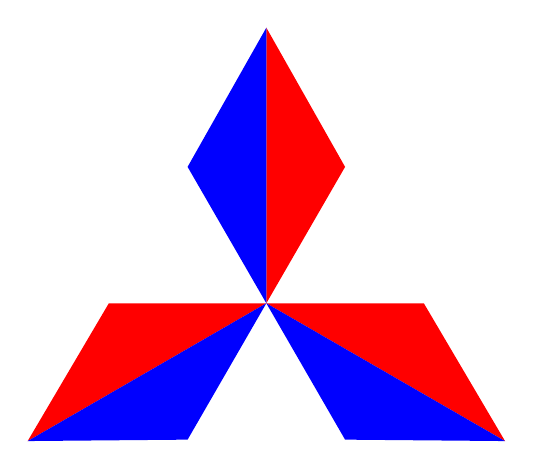
\begin{tikzpicture}			
		% Diamond 1		
		\fill[red] (0,0) -- (0:2) -- (-30:3.5);
		\fill[blue] (0,0) -- (-60:2) -- (-30:3.5);
		
		\fill[red] (0,0) -- (0:-2) -- (30:-3.5);
		\fill[blue] (0,0) -- (60:-2) -- (30:-3.5);	
		
		\fill[red] (0,0) -- (60:2) -- (90:3.5);
		\fill[blue] (0,0) -- (-60:-2) -- (90:3.5);			
	\end{tikzpicture}	
\end{document}